\section{Thesis Outline}\label{sec:introduction:outline}

\begin{figure}[ht]
    \centering
    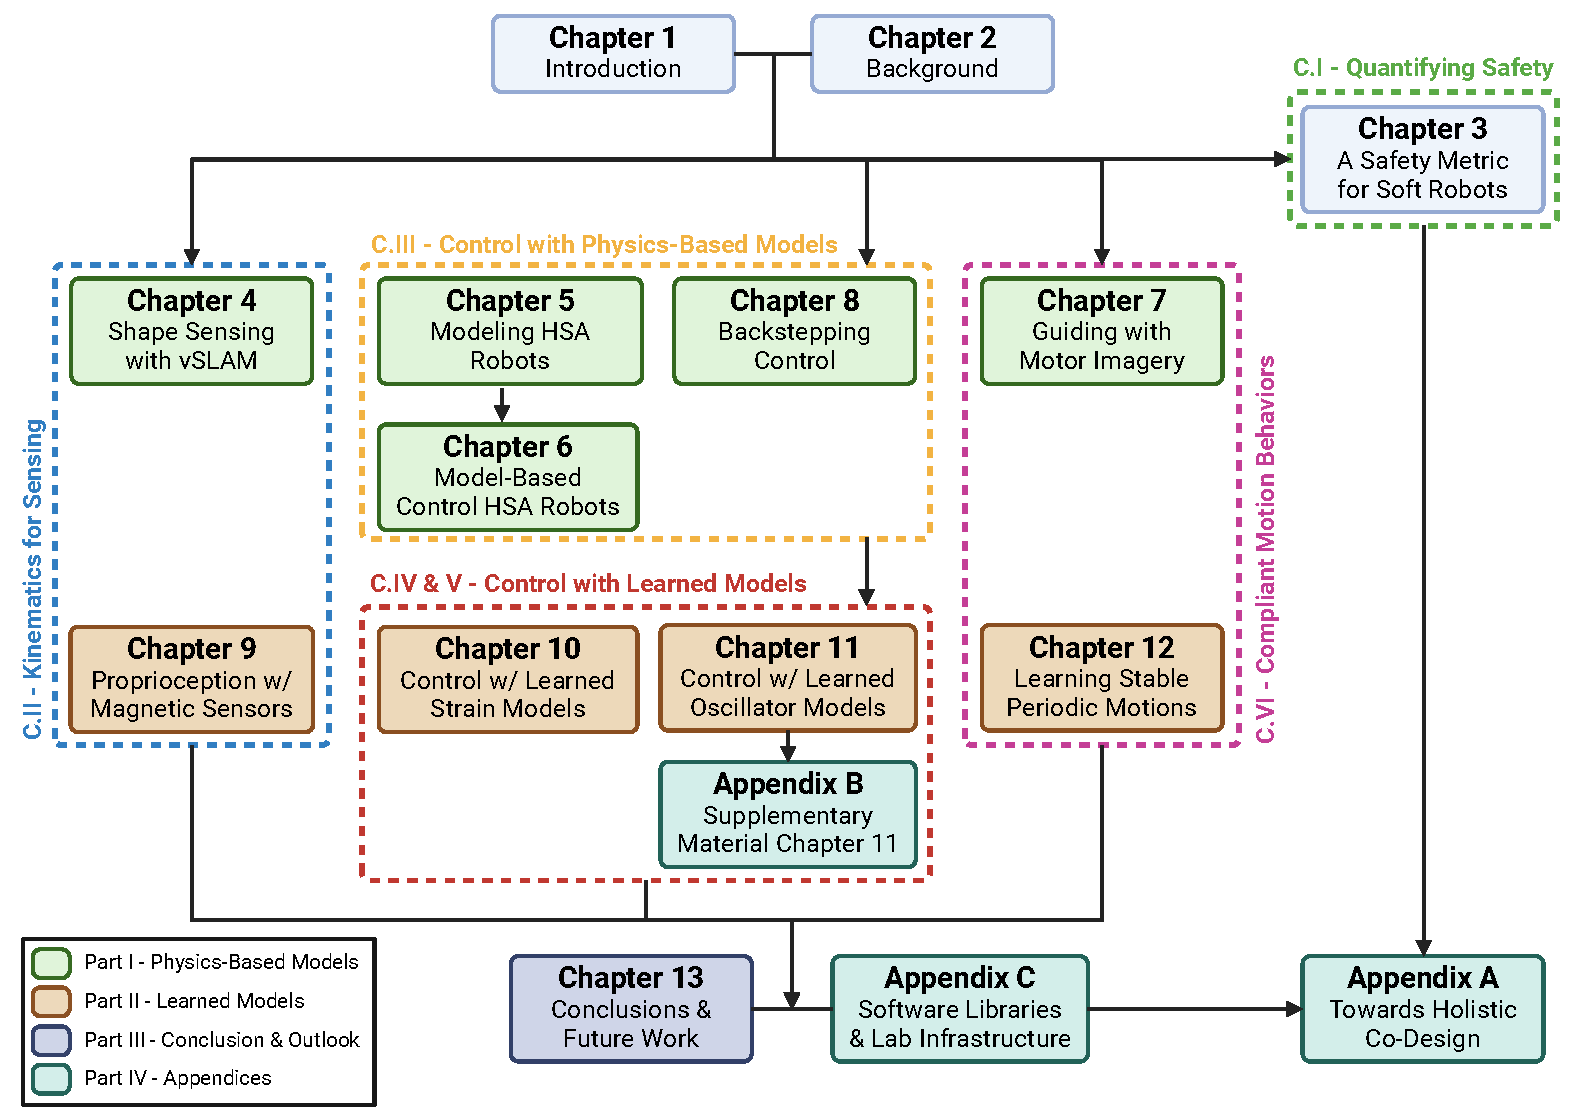
\includegraphics[width=1.0\linewidth]{introduction/figures/thesis_outline_tree_v2.pdf}
    \caption{Outline of this thesis with a focus on the contributions. The background colors of the blocks refer to the parts of this thesis. With \emph{C.X}, we refer to the various contributions with dashed frames encapsulating the corresponding chapters.}
    \label{fig:introduction:thesis_outline_tree}
\end{figure}

\begin{figure}[ht]
    \centering
    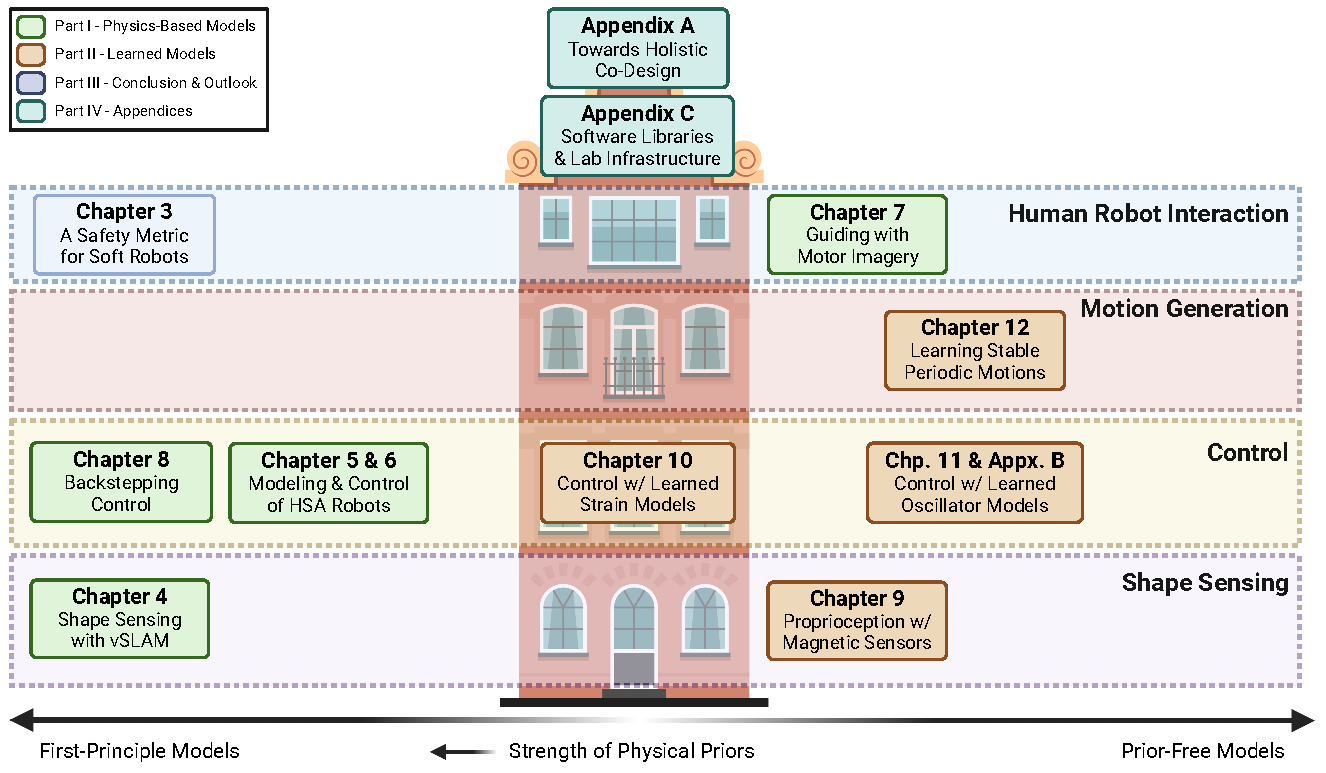
\includegraphics[width=1.0\linewidth]{introduction/figures/thesis_outline_house_v2.pdf}
    \caption{Outline of this thesis with a focus the physical priors of the models and the application area of the model (e.g., proprioception/shape sensing, control, motion generation/policies, and \gls{HRI}).}
    \label{fig:introduction:thesis_outline_house}
\end{figure}

In the following, we will outline the structure of this thesis, which is also visualized in Figs.~\ref{fig:introduction:thesis_outline_tree}-\ref{fig:introduction:thesis_outline_house}.

% In Chapter~\ref{chp:background}, we provide background on the existing work on kinematic parametrizations of the backbone shape of soft robots, the derivation of the forward kinematics, and dynamical model~\citep{armanini2023soft, alessi2024rod}. Finally, we reference established model-based control approaches for continuum soft robots.
Chapter~\ref{chp:background} aims to provide background on the existing literature on modeling and control of soft robots and introduce specific kinematic and dynamic models, controllers, and other concepts that are reoccurring throughout this thesis
For example, this includes the \gls{PCS} kinematic parametrization, Euler-Lagrangian dynamic models of soft robots, and P-satI-D~\citep{pustina2022p}+potential shaping~\citep{della2023model} controllers.

Chapter~\ref{chp:safetymetric} incorporating Contribution~\ref{contrib:safety_metric} analyzes the inherent safety of soft robots and recognizes the need for a quantitative safety metric that encompasses both the embodied and computational intelligence of the robotic system. After identifying interesting applications of a safety metric, we devise the requirements such a metric would need to meet. We then propose the first quantitative safety metric for soft robotic manipulators. Finally, we give recommendations for the safe design of soft robotic systems.

% At the outset of working on this thesis, there was still a lack of understanding of some fundamental characteristics of the behavior of soft robots.
% Examples include (1) detailed knowledge about the actuation behavior, such as the coupled dynamics between soft robots and pneumatic piston actuators or the transfer of power from electric actuators through an auxetic metamaterial to a deformation of the overall structure as is the case for \gls{HSA} robots, (2) or kinematic parametrizations that can selectively keep specific strains (e.g., bending, twist, axial) constant or piecewise constant over the backbone discretization.
% Therefore, we decided to dedicate a significant part of this thesis to advancing our understanding of soft robotic behavior by modeling these effects and dynamics using physics-based approaches, subsequently experimentally verifying them, and finally exploiting this gained model knowledge for improving the shape sensing and model-based control of soft robots.
% This content is contained in Part~\ref{part:physicsmodels}, where we present advanced physics-based models for shape sensing and model-based control.
At the outset of this thesis, our understanding of several fundamental aspects of soft robot behavior was still limited. For instance, we lacked detailed insights into actuation dynamics~\citep{della2023model}—such as the coupled behavior between soft robots and pneumatic piston actuators or how power is transmitted from electric actuators through auxetic metamaterials to induce deformations in \gls{HSA} robots—as well as in kinematic parameterizations that allow for an optimal tradeoff between dimensionality and expressiveness - as ones that maintain specific strains, such as bending, twist, axial, either constant or piecewise constant along the backbone. Consequently, we devoted a significant portion of this thesis to advancing our understanding by developing physics-based models, experimentally validating them, and leveraging the results to enhance shape sensing and model-based control. This work is presented in Part~\ref{part:physicsmodels}, where we introduce advanced physics-based models for these two applications.

% This better understanding of advanced soft robot characteristics gave us the necessary know-how to propose better-suited physical priors for integrating into learned models.
% Specifically, Part~\ref{part:learning} is dedicated to incorporating priors related to kinematics, stability characteristics, and physical structure into \gls{ML}-based methods, utilizing these hybrid models for shape sensing and control. The content of both parts is discussed in greater detail below. Finally, in Chapter~\ref{chp:conclusion}, we summarize our findings and suggest promising directions for future research.
This deeper insight into soft robot characteristics has equipped us to propose more suitable physical priors for integration into learned models. Specifically, Part~\ref{part:learning} focuses on incorporating priors related to kinematics, stability, and physical structure into \gls{ML}-based methods, thereby employing these hybrid models for improved shape sensing and control. 

Parts~\ref{part:physicsmodels} \& \ref{part:learning} are discussed in further detail in the following subsections.

\subsection*{Part I - Shape Sensing and Control with Advanced Physics-based Models}

% In Part~\ref{part:physicsmodels}, we derive advanced physics-based models of soft robots and exploit them for shape sensing and control.
% Specifically, we as i) leverage project pose estimates stemming from \gls{SLAM} algorithms onto a kinematic model to increase the performance of shape sensing based on visual sensors, ii) develop kinematic and dynamic models for \gls{HSA} robots, and subsequently exploit them for model-based control, iv) propose a motor-imagery-based \glsxtrfull{BCI} interface for guiding a low-level impedance controller with brain signals, and v) model the actuation dynamics of pneumatic piston-driven soft robots and devise a provably-stable backstepping controller for regulating the motion of the piston.
% This part contains Contributions~\ref{contrib:kinematic_models_shape_sensing}-\ref{contrib:model_based_control_with_learned_models} and is composed of the following chapters:
In Part~\ref{part:physicsmodels}, we develop advanced physics-based models for soft robots and apply them to shape sensing and control. Specifically, we: i) enhance shape sensing based on visual sensors by leveraging pose estimates from \gls{SLAM} algorithms and projecting them onto a kinematic model, ii) propose kinematic and dynamic models for \gls{HSA} robots and utilize them for model-based control, iii) introduce a motor-imagery-based \glsxtrfull{BCI} interface for guiding a low-level impedance controller with brain signals, and iv) model the actuation dynamics of pneumatic piston-driven soft robots, designing a provably stable backstepping controller for piston motion regulation.
%
This part includes Contributions~\ref{contrib:kinematic_models_shape_sensing}-\ref{contrib:model_based_control_with_learned_models} and comprises the following chapters:

\begin{itemize}
    % \item \textbf{Chapter~\ref{chp:srslam}} presents a methodology for combining low-cost monocular cameras with \gls{vSLAM} algorithms and a projection of pose estimates onto the kinematics of the soft robot to achieve shape sensing for soft robots. The approach is verified in both simulations with a \gls{CC} model and experimentally with a pneumatic soft robot segment moving in 3D space.
    \item \textbf{Chapter~\ref{chp:srslam}} describes a method for combining low-cost monocular cameras with \gls{vSLAM} algorithms and projecting pose estimates onto the soft robot’s kinematics to enable shape sensing. The approach is validated through simulations using a \gls{CC} model and experimental tests on a pneumatic soft robot segment moving in 3D space.
    % \item \textbf{Chapter~\ref{chp:hsamodel}} proposes kinematic, dynamic, and actuation models for \gls{HSA} robots consisting of parallel auxetic metamaterial rods. Firstly, we propose a new kinematic parametrization (\gls{SPCS}) based on the \gls{PCS}~\citep{renda2018discrete} model that is able to capture the shape of \gls{HSA} rods using the least possible configuration variables.  Secondly, we establish a formalism for incorporating the auxetic trajectory (e.g., \gls{HSA} rods changing length in the presence of twist strains) into Cosserat rod-based models, which enables a PyElastica~\citep{naughton2021elastica}-based simulator for \gls{HSA} robots. Subsequently, we devise a kinematic model for planar \gls{HSA} robots by approximating its virtual backbone with \gls{CS}. Finally, we devise for the planar case an underactuated dynamical model in Euler-Lagrangian form that considers the particular characteristics of \gls{HSA} robots, such as the auxetic trajectory of the \glspl{HSA}, which causes rest length and stiffness of the robot to vary as a function of the twist strain. All devised models are experimentally verified. 
    \item \textbf{Chapter~\ref{chp:hsamodel}} presents kinematic, dynamic, and actuation models for \gls{HSA} robots comprising parallel auxetic metamaterial rods. First, we introduce a novel kinematic parametrization (\gls{SPCS}) based on the \gls{PCS}~\citep{renda2018discrete} model, effectively capturing \gls{HSA} rod shapes with minimal configuration variables. Next, we formalize the inclusion of auxetic trajectories (e.g., \gls{HSA} rods changing length with twist strains) in Cosserat rod-based models, enabling a PyElastica~\citep{naughton2021elastica}-based simulator for \gls{HSA} robots. Additionally, we devise kinematic and underactuated dynamic models for planar \gls{HSA} robots, incorporating auxetic trajectories that influence rest length and stiffness. These models are experimentally validated.  
    % \item \textbf{Chapter~\ref{chp:hsacontrol}} builds upon Chapter~\ref{chp:hsamodel} by devising two model-based control approaches for setpoint regulation with planar \gls{HSA} robots: a) a configuration-space controller consists of an integral-saturated PID controller as the feedback term and a potential shaping feedforward term, b) a operational space impedance controller that allows shaping of the closed-loop end-effector stiffness in Cartesian space through a PD feedback term. The configuration-space controller in a) is enabled by a feedforward term that evaluates the potential forces at the desired end-effector position via static inversion and ii) a feedback term that is enabled by a combination of approaches, such as linearization and mapping into actuation coordinates, to make the actuation term more control friendly. The operational space impedance controller in b) relies upon canceling the existing soft robot dynamics using the model knowledge and solving the underactuated mapping from configuration-space torques onto control inputs with a least-squares optimizer. The control approaches are extensively verified experimentally and benchmarked against a model-free PID controller.
    \item \textbf{Chapter~\ref{chp:hsacontrol}} extends Chapter~\ref{chp:hsamodel} by proposing two model-based control strategies for setpoint regulation with planar \gls{HSA} robots: a) a configuration-space controller using an integral-saturated PID feedback term and potential shaping feedforward term, and b) an operational space impedance controller that enables end-effector stiffness shaping in Cartesian space through a PD feedback term. The configuration-space controller leverages a feedforward term evaluating potential forces at desired end-effector positions via static inversion and a feedback term enabled by linearization of the actuation term and mapping into collocated form. The operational space controller uses model knowledge to cancel the existing soft robot dynamics and applies a least-squares optimizer to solve the underactuated control problem (i.e., mapping configuration space torques to actuation inputs). Both approaches are extensively validated experimentally and benchmarked against a model-free PID controller.  
    % \item \textbf{Chapter~\ref{chp:braincontrol}} augments the operational space impedance control from Chapter~\ref{chp:hsacontrol} with a \gls{BMI} protocol that allows a user to operate a soft robot by imagining motor movements. The \gls{BMI} protocol transforms measurements by a wearable \gls{EEG} device into spatial movements of an end-effector attractor by first classifying them using \gls{LDA} and subsequently translating the motor imagery into an incremental movement of the attractor along the coordinate axes. The impedance controller subsequently tracks the setpoints. We experimentally, with a planar \gls{HSA} robot, compare the control performance of the proposed approach on a reference trajectory of nine-step functions against two baselines: a) computational control, where the impedance controller directly has access to the privileged goal information, and b) control using a much more established \gls{HRI} interface - a keyboard. Finally, we take a first foray into assisting humans with a simple \gls{ADL} - releasing hairspray from a bottle by guiding the soft robot using motor imagery to exert force on the button with its end-effector.
    \item \textbf{Chapter~\ref{chp:braincontrol}} enhances the operational space impedance controller from Chapter~\ref{chp:hsacontrol} with a \gls{BMI} protocol, enabling users to control a soft robot through motor imagery. The protocol processes wearable \gls{EEG} device measurements, classifies motor imagery using \gls{LDA}, and translates the output into incremental end-effector attractor movements. The low-level impedance controller then tracks these setpoints. Experiments with a planar \gls{HSA} robot compare this approach's performance on a reference trajectory against two baselines: a computational control with privileged access to goal positions and a keyboard-based \gls{HRI} interface. Finally, we demonstrate a simple \gls{ADL}—releasing hairspray by guiding the soft robot to press a button using motor imagery.  
    % \item \textbf{Chapter~\ref{chp:backstepping}} models the actuation dynamics of a pneumatic piston-driven soft robot and subsequently exploits the model knowledge to devise a nonlinear controller for the actuation of the piston by following a backstepping approach~\citep{kokotovic1992joy, lozano1992adaptive, khalil2002nonlinear}. The model is enabled by formulating the potential energy stored in the fluid as a function of the soft robot configuration and the position of the piston. Its partial derivative then represents the potential forces that fluid exerts on the piston and the soft robot, respectively. The backstepping controller integrates a configuration-space setpoint regulator into a feedback controller for the pistons. The proposed approach is tested in simulation on a three-segment \gls{PCC} soft robot.
    \item \textbf{Chapter~\ref{chp:backstepping}} develops dynamic models of the actuation dynamics for pneumatic piston-driven soft robots and designs a nonlinear backstepping controller~\citep{kokotovic1992joy, lozano1992adaptive, khalil2002nonlinear}. The model calculates the potential energy stored in the fluid as a function of the robot's configuration and piston position, with partial derivatives representing the potential forces exerted by the fluid. The backstepping controller integrates a configuration-space setpoint regulator into a piston feedback controller. This approach is tested through simulations on a three-segment \gls{PCC} soft robot.  
\end{itemize}

\subsection*{Part II - Incorporating Physical Structure and Stability Guarantees into Learned Models and Controllers}

% Part~\ref{part:learning} encompasses various pieces of research where we combine modern \gls{ML} approaches with physics models with the aim of simplifying the learning problem, enabling insight into the learned component by establishing a physical interpretation, adding stability guarantees, and/or exploiting a physical structure for model-based control with energy-shaping approaches. It touches Contributions~\ref{contrib:kinematic_models_shape_sensing},\ref{contrib:learned_models}-\ref{contrib:motion_behaviors} and contains the following chapters
Part~\ref{part:learning} combines several research efforts integrating modern \gls{ML} techniques with physics-based models. The goal is to simplify the learning process, provide insights into the learned components through physical interpretation, ensure stability guarantees, and/or leverage physical structures for model-based control using energy-shaping approaches. This part covers Contributions~\ref{contrib:kinematic_models_shape_sensing},\ref{contrib:learned_models}-\ref{contrib:motion_behaviors} and includes the following chapters:

\begin{itemize}
    % \item \textbf{Chapter~\ref{chp:promasens}} develops a methodology to achieve shape sensing for 3D soft robots by embedding multiple magnets and magnetic sensors into the body.
    % The main challenge connected with magnetic sensors is interpreting their measurements and mapping them onto a configuration estimate. 
    % We leverage the kinematic model of the soft robot to parameterize the spatial relation between a magnetic sensor and its surrounding magnets. We then learn the forward measurement model from this low-dimensional parametrization to predicted measurements of each sensor. Interestingly, as we reduced the size of the learning \emph{black-box} by exploiting kinematic model knowledge, this learned sensor measurement model generalizes across all embedded magnetic sensors.
    % Finally, to achieve proprioception, we formulate an optimization problem with the cost function being the squared error between the predicted and actual sensor measurements. As both the kinematics and the neural sensor measurement predictor are analytically differentiable, we can efficiently solve this optimization problem using gradient descent. We verify the proposed approach both in simulation with \gls{PCC} and \gls{PAC} soft robots and experimentally with a pneumatically actuated soft segment.
    \item \textbf{Chapter~\ref{chp:promasens}} presents a methodology for achieving 3D shape sensing in soft robots by embedding multiple magnets and magnetic sensors within their body. The primary challenge with magnetic sensors lies in interpreting their measurements and mapping them to a configuration estimate. To address this, we use the kinematic model of the soft robot to parameterize the spatial relationship between a magnetic sensor and its surrounding magnets. We then learn the forward measurement model based on this low-dimensional parameterization to predict the measurements for each sensor. Notably, by incorporating knowledge of the kinematic model and reducing the complexity of the learning \emph{black-box}, the resulting sensor measurement model generalizes effectively across all embedded magnetic sensors. Finally, to achieve proprioception, we formulate an optimization problem where the cost function minimizes the squared error between predicted and actual sensor measurements. With both the kinematic model and the neural sensor measurement predictor being analytically differentiable, this optimization problem is efficiently solved using gradient descent. The proposed approach is validated through simulations with \gls{PCC} and \gls{PAC} soft robots, as well as experiments with a pneumatically actuated soft segment.
    % \item \textbf{Chapter~\ref{chp:pcsregression}} presents an algorithmic approach for identifying low-dimensional strain models based on data describing the shape evolution of soft robots. The approach assumes as inputs pose measurements along the soft robot's backbone, and it consists of two steps: First, we identify a suitable low-dimensional \gls{PCS}-based parametrization that can approximate the backbone shape well using an iterative procedure. Subsequently, a dynamical model is derived based on the kinematic parametrization, and its parameters are regressed in closed form. Furthermore, the algorithm leverages heuristics such as the identified stiffness to decide if some strains can be neglected and, with that, if the \gls{DOF} of the dynamical model can be further reduced. We verify the proposed approach by identifying the dynamical model directly from videos of a simulated soft robot. We quantitatively benchmark the performance of the derived model against \gls{SOTA} \gls{ML} approaches such as \glspl{RNN}, \glspl{NODE}, etc., and demonstrate how learning this fully physics-based strain model offers much-improved extrapolation performance when tested on outside of the training set actuation sequences. Finally, we leverage the learned model for model-based control with the controller containing an integral-saturated PID feedback term and a potential shaping feedforward term - a similar control approach as applied in Chapter~\ref{chp:hsacontrol}.
    \item \textbf{Chapter~\ref{chp:pcsregression}} introduces an algorithmic framework for identifying low-dimensional strain models from data describing the shape evolution of soft robots. The approach takes as input pose measurements along the soft robot’s backbone and consists of two key steps: First, a suitable low-dimensional \gls{PCS}-based parameterization is identified through an iterative procedure to approximate the backbone shape accurately. Next, a dynamical model is derived from this kinematic parameterization, with its parameters regressed in closed form. Additionally, the algorithm employs heuristics, such as the identified stiffness, to determine whether certain strains can be neglected, potentially further reducing the \gls{DOF} of the dynamical model. The proposed method is validated by deriving the dynamical model of a simulated soft robot directly from video data. Its performance is quantitatively benchmarked against \gls{SOTA} \gls{ML} approaches, including \glspl{RNN} and \glspl{NODE}. Results demonstrate that this fully physics-based strain model significantly outperforms others in extrapolation settings, particularly for actuation sequences outside the training set. Finally, the learned model is employed for model-based control using a controller that incorporates an integral-saturated PID feedback term alongside a potential-shaping feedforward term, similar to the control approach outlined in Chapter~\ref{chp:hsacontrol}.
    % \item \textbf{Chapter~\ref{chp:con}} proposes to learn the latent dynamics of physical systems, such as soft robots, using Coupled Oscillator Networks (CONs). Specifically, this means that we map high-dimensional observations, such as images of the soft robot, into a low-dimensional latent space with a learned autoencoder. The latent space now possesses a mechanical interpretation as each latent variable corresponds to the position of a mechanical oscillator. One benefit of this strategy is that the presented formulation of \gls{CON} exhibits strong stability guarantees as the unactuated system is \glsxtrfull{GAS} and the actuated system \glsxtrfull{ISS}~\citep{khalil2002nonlinear}. We verify the learning approach, among others, on multiple datasets containing image sequences of the motion of simulated soft robots and benchmark the motion prediction accuracy against various \gls{SOTA} \gls{ML} approaches such as \gls{coRNN}, \gls{GRU}, etc.
    % Even more importantly, we can leverage the physical structure of the \gls{CON} dynamics for closed-form model-based feedback control in latent space. Again, we use here an integral-saturated PID as the feedback term and reshape the potential field of \gls{CON} to have its minimum at the desired latent goal. We verify the proposed control strategy on a simulated two-segment \gls{PCC} soft robot.
    \item \textbf{Chapter~\ref{chp:con}} introduces a method for learning the latent dynamics of physical systems, such as soft robots, using Coupled Oscillator Networks (CONs). Specifically, high-dimensional observations, like images of the soft robot, are mapped into a low-dimensional latent space using a learned autoencoder. Each latent variable in this space corresponds to the position of a mechanical oscillator, providing a clear mechanical interpretation. A key advantage of this approach is that the \gls{CON} formulation offers strong stability guarantees: the unactuated system exhibits \glsxtrfull{GAS}, while we prove for the actuated system \glsxtrfull{ISS}~\citep{khalil2002nonlinear}. The proposed learning method is validated on multiple datasets comprising image sequences of simulated soft robot motions, and its motion prediction accuracy is benchmarked against various \gls{SOTA} \gls{ML} approaches, such as \gls{coRNN} and \gls{GRU}. Furthermore, the physical structure of the \gls{CON} dynamics is leveraged for closed-form model-based feedback control in the latent space. This involves using an integral-saturated PID feedback term and reshaping the \gls{CON} potential field to exhibit its minimum at the desired latent goal. The proposed control strategy is demonstrated on a simulated two-segment \gls{PCC} soft robot.
    % \item \textbf{Chapter~\ref{chp:osmp}} puts forward a method for learning orbitally stable motion policies from demonstration that can be used as a reference to the low-level motor controller presented, for example in Chapters~\ref{chp:hsacontrol} \& \ref{chp:pcsregression} - \ref{chp:con}. Specifically, we build on the existing pioneering research on \glsxtrfull{SMP} that parametrizes motion policies with (latent) dynamical systems~\citep{ijspeert2013dynamical, rana2020euclideanizing}. In this chapter, we combine a learned bijective encoder implemented as a Euclideanizing flow~\citep{dinh2016density, rana2020euclideanizing} with an orbitally stable supercritical Hopf bifurcation as the latent dynamics to learn periodic motions from demonstrations with stability guarantees.
    % The inverse Jacobian of the bijective encoder allows the projection of predicted latent velocities back into the oracle space. We validate the approach experimentally on multiple robot embodiments, such as a tendon-driven helicoid soft robot~\citep{guan2023trimmed}, a swimming turtle robot, a UR5 robotic manipulator, and a Kuka \gls{Cobot}.
    \item \textbf{Chapter~\ref{chp:osmp}} proposes a method for learning orbitally stable motion policies from demonstration, which can serve as a reference for the low-level motor controllers introduced in Chapters~\ref{chp:hsacontrol} and \ref{chp:pcsregression}–\ref{chp:con}. Building on pioneering research in \glsxtrfull{SMP}, which parameterizes motion policies using (latent) dynamical systems~\citep{ijspeert2013dynamical, rana2020euclideanizing}, this chapter integrates a learned bijective encoder implemented as a Euclideanizing flow~\citep{dinh2016density, rana2020euclideanizing} with an orbitally stable supercritical Hopf bifurcation as the latent dynamics. This approach enables the learning of periodic motions from demonstrations with stability guarantees. The inverse Jacobian of the bijective encoder facilitates the projection of predicted latent velocities back into the oracle space. The proposed method is experimentally validated on various robot embodiments, including a tendon-driven helicoid soft robot~\citep{guan2023trimmed}, a swimming turtle robot, a UR5 robotic manipulator, and a Kuka \gls{Cobot}.
\end{itemize}

\subsection*{Conclusion and Appendices}
In the following, we will detail the content of Parts~\ref{part:conclusion} \& \ref{part:appendices} \ref{part:appendices}.
\begin{itemize}
    \item \textbf{Chapter~\ref{chp:conclusion}} summarizes our findings and suggests promising directions for future research.
    \item 
    % \textbf{Appendix~\ref{chp:apx:holisticcodesign}} proposes a framework for holistic co-design of soft robots that enables co-optimization of soft robot body (e.g., its morphology) and brain (e.g., perception and control systems)~\citep{spielberg2019learning, wang2024diffusebot, navez2024contributions}. Crucially, this framework considers a broad set of values beyond task-centric performance, such as safety, manufacturability, and regulatory considers, it explicitly accounts for realization of the design and how prototyping can decrease the uncertainty in the evaluation metrics used to assess designs computationally, and it proposes modifications and augmentations to the co-design process that have the potential to make it computationally significantly more efficient. In summary, this holistic co-design framework guides a way towards how the soft robot's structural shape, the actuator and sensing placement (see Chapters~\ref{chp:srslam} \& \ref{chp:promasens}), the reduced-order modeling (see Chapters~\ref{chp:hsamodel}, \ref{chp:pcsregression}, \& \ref{chp:con}), and the controller (see Chapters~\ref{chp:hsacontrol}, \ref{chp:backstepping}, \ref{chp:pcsregression}, \& \ref{chp:con}) could be jointly optimized in the future to optimize performance while ensuring that the closed-loop system remains sufficiently compliant and safe (see Chapter~\ref{chp:safetymetric}).
    \textbf{Appendix~\ref{chp:apx:holisticcodesign}} introduces a framework for the holistic co-design of soft robots, enabling the simultaneous optimization of both the robot’s body (e.g., its morphology) and its brain (e.g., the perception and control systems)~\citep{spielberg2019learning, wang2024diffusebot, navez2024contributions}. Importantly, the framework considers a broad array of criteria beyond task-centric performance, including safety, manufacturability, and regulatory considerations. It explicitly addresses the practical realization of designs by demonstrating how prototyping can reduce uncertainty in the computational evaluation metrics, while also proposing modifications to the co-design process that could greatly enhance computational efficiency. In summary, this holistic co-design framework provides guidance on how the soft robot’s structural shape, actuator and sensor placement (see Chapters\ref{chp:srslam} \& \ref{chp:promasens}), reduced-order modeling (see Chapters~\ref{chp:hsamodel}, \ref{chp:pcsregression}, \& \ref{chp:con}), and controller (see Chapters~\ref{chp:hsacontrol}, \ref{chp:backstepping}, \ref{chp:pcsregression}, \& \ref{chp:con}) might be jointly optimized in the future to boost performance while ensuring that the closed-loop system remains sufficiently compliant and safe (see Chapter~\ref{chp:safetymetric}).
    \item \textbf{Appendix~\ref{chp:apx:con}} contains supplementary material, including details on the experimental setup and additional results, for Chapter~\ref{chp:con}.
    \item 
    % \textbf{Appendix~\ref{chp:apx:infrastructure}} details some of the lab infrastructure, such as a motion capture system and pneumatic pressure regulation, that was developed as part of this PhD to support and enable the research presented in this thesis. Furthermore, we present some of the software libraries that support many of the chapters contained in this thesis. For example, a JAX implementation of control-oriented soft robot models that enables simulation, model-based control, or in the future motion planning, or a ROS2 ecosystem for the control of \gls{HSA} robots.
    \textbf{Appendix~\ref{chp:apx:infrastructure}} outlines some of the laboratory infrastructure developed during this PhD—such as a motion capture system and pneumatic pressure regulation—to support the research presented in this thesis. Additionally, we introduce several software libraries that underpin many of the thesis chapters, including a JAX implementation of control-oriented soft robot models for simulation, model-based control, and motion planning, as well as a ROS2 ecosystem for model-based control of \gls{HSA} robots.
\end{itemize}
 

\subsection{Important Notes}
% We note that while we aimed to keep the notation similar throughout the chapters, the variety of problem settings and methods combined with the limited number of available symbols allowed us to develop tailored notations for each chapter.
We acknowledge that, although we strived to maintain consistent notation across chapters, the diversity of problem settings and methods, coupled with the limited pool of available symbols, necessitated the use of tailored notations for each chapter.
% Also, please note that in the following, if not explicitly otherwise noted, we refer with the expression \emph{soft robot} to \emph{continuum soft robots} (versus articulated soft robots)~\cite{della2020softencyclopedia}.
Please note that, unless explicitly stated otherwise, the term "soft robot" in this thesis refers to "continuum soft robots" (as opposed to articulated soft robots)~\citep{della2020softencyclopedia}.